\section{Background: Knowledge Distillation}

\subsection{Problem statement}
Neural network models have been successful in a myriad of fields including extremely complex problems. However, these models are enormous in size and computational hungry, thus cannot be deployed to on-edge devices nor feasibly runnable in some situations. To compensate for this situation, knowledge distillation was first proposed in \cite{firstkdpaper} and properly formalize in \cite{hintonfirstkd}. In the work of Buciluǎ et al. \cite{firstkdpaper}, the knowlegde is transferred from the larger model to the smaller model while minimizing the logits difference produced by those two models respectively. This vanilla method opened the first path of knowledge type that can be used to distilled, later on, there started to have some other works using the activations, feature maps of intermediate layers as the guide for the student network \cite{featurebased01, featurebased02_AT,featurebased03_relu}. Some other methods to extract knowledge by comparing the relationship between different layers of teacher model \cite{relbase01, relbase02} are also worth mentioning but won't be discussed in this survey.
%-------------------------------------------------------------------------
\begin{table*}[h]
   \begin{center}
      \begin{tabular}{|l|l|l|c|}
         \hline
         Paper                & Main motives               & Description                           & Year \\ \hline
         \cite{logitable01}   & Enhance distilling process & \begin{tabular}[c]{@{}l@{}}Train in generation, control the strictness \\ while training teacher network \\ (adding extra loss term)\end{tabular}             & 2018 \\ \hline
         \cite{logitable10}   & Enhance distilling process & \begin{tabular}[c]{@{}l@{}}Propose Stage-by-Stage Knowledge Distillation:\\ 2 separated parts: backbone \\ (mimics the output feature of teacher progressively) \\ and task-head (only use ground-truth label).\end{tabular}             & 2018 \\ \hline
         \cite{logitable12}   & \begin{tabular}[c]{@{}l@{}}Enhance distilling process\\ Novel distillation framework\end{tabular}  & \begin{tabular}[c]{@{}l@{}}Propose distillation framework \\ allowing teacher and student \\ having the same architecture, the framework also use \\ the same architecture for both model \\ since it use model from the previous iteration.\end{tabular}             & 2018 \\ \hline
         \cite{logitable03}   & Enhance distilling process & \begin{tabular}[c]{@{}l@{}}Proposed new loss function \\ while extracting relational information \\ using a relational potential function\end{tabular}             & 2019 \\ \hline
         \cite{teacherfree}   & \begin{tabular}[c]{@{}l@{}}Learn from noisy data\\ Novel distillation framework\end{tabular}  & \begin{tabular}[c]{@{}l@{}}Propose Teacher-free distillation framework:\\ including self-training and self-regularization\end{tabular}             & 2020 \\ \hline
         \cite{logitable11}   & Enhance distilling process & \begin{tabular}[c]{@{}l@{}}Allow student to selectively choose to learn \\ from either the teacher model or the ground truth \\ conditioned on whether the teacher can correctly \\ predict the truth rather than using interpolated labels\end{tabular}             & 2019 \\ \hline
         \cite{complexitygap} & Enhance distilling process & Using early stopping as a regularizer & 2019 \\ \hline
         \cite{logitable04}   & Enhance distilling process & \begin{tabular}[c]{@{}l@{}}In order to minimize the complexity gap, \\ proposed a multi-step distillation.\end{tabular}             & 2019 \\ \hline
         \cite{logitable05}   & Ensemble of distribution   & \begin{tabular}[c]{@{}l@{}}Distill the distribution of the predictions \\ from an ensemble so that student can \\ receive both the enhanced \\ prediction and diversity\end{tabular}            & 2020 \\ \hline
         \cite{logitable06}   & \begin{tabular}[c]{@{}l@{}}Add Regularization\\ Ensemble of distribution\\ Learn from noisy data\end{tabular} & \begin{tabular}[c]{@{}l@{}}Injecting different type of noises \\ during the distillation process: \\ 1) Dropout while distilling \\ 2) training student with noisy data \\ while teacher had been trained on clean data \\ 3) Randomly change true labels to random target \\ by an uniform distribution\end{tabular}            & 2020 \\ \hline
         \cite{logitable07}   & \begin{tabular}[c]{@{}l@{}}Enhance distilling process\\ Learn from noisy data\end{tabular} & \begin{tabular}[c]{@{}l@{}}Generate pseudo labels for unlabeled images then \\ train student model on those while injecting noises: \\ dropout, data augmentation\end{tabular}            & 2020 \\ \hline
         \cite{logitable08}   & \begin{tabular}[c]{@{}l@{}}Add Regularization\\ Enhance distilling process\end{tabular} & \begin{tabular}[c]{@{}l@{}}1) Minimizing genetic error: Using Label Smoothing \\ Regularizer and propose new loss which tries to \\ adjust the teacher's prediction w.r.t. ground truth labels\\ 2) Dynamic temperature distillation: \\ tuning $\tau$ sample\end{tabular}            & 2020 \\ \hline
         \cite{logitable09}   & \begin{tabular}[c]{@{}l@{}}Add Regularization\\ Enhance distilling process\end{tabular} & \begin{tabular}[c]{@{}l@{}}Apply margin-based softmax \\ and normalize input vector/ weight matrix\\ so that student model con focuses on \\ samples with more confident predictions\end{tabular}            & 2020 \\ \hline
      \end{tabular}
   \end{center}
   \label{tab:logitbased_related}
\end{table*}

\subsection{Knowledge}
\subsubsection{Knowledge from logits}
   
This type of knowledge extraction usually refers to using the neural response of the final output layer, or also known as \textit{logits} of the teacher model. As stated before, the first application of logits in KD is used in \cite{firstkdpaper}, but in many situations, given a highly confident teacher model, the output of softmax function gives more or less the same information as the ground truth label (since this is the core idea of softmax function - maximizing the probabilities of one while minimizing the others). Tackling this problem, Hinton et al. \cite{hintonfirstkd} proposed the concept of 'soft labels' and declared that this type of label contains informative \textit{dark knowledge}. Given the \textbf{logits} $z$ from a network, the 'soft label' $p_i$ of an image is defined as:
\[
   p_i = \frac{\text{exp}(\frac{z_i}{\rho})}{\sum_j \text{exp}(\frac{z_i}{\rho})}
\]
where $\rho$ is the temperature parameter, notice that when $\rho=1$, we get the normal softmax function. Determine which value is optimal for $\rho$ is still a debatable topics but it is argued that while increasing $\rho$, the label becomes softer and providing more information about which class is similar to the predicted label. Accordingly, the logits-based distillation loss function is defined as follow:
\[
   \mathcal{L}_{\text{LB}}(x;\theta) = \alpha * \mathcal{H}(y, \sigma(z_s)) + \beta * \mathcal{H}(\sigma(z_t;\rho), \sigma(z_s;\rho))
\]
where $x$ is the input, $\theta$ are the student model weights, $\mathcal{H}(.)$ is the cross-entropy loss function, $y$ is the ground truth label, $\sigma(.)$ is the $\rho$-parameterized softmax function, $\alpha, \beta$ are the coefficients to tune in order to balance between both cross-entropies, and $z_t, z_s$ are the logits of teacher and student model respectively. Figure \ref{fig:logits_base} illustrate an usual framework while using this type of knowledge.

Logits-based knowledge is fairly straightforward and easy to implement so it is often the first approach used when need to apply knowledge distillation. As far as the survey goes, there are several main motives of using logits-based knowledge: 1) using soft labels with regularization 2) create/use noisy data to train 3) enhancement. A brief table containing its descriptions and several related work can be found at \ref{tab:logitbased_related}. Nevertheless, since this type of knowledge only utilizes the final output of the teacher model, it fails to offer information gathered in the intermediate layers, which later was proved to contain many informative results \cite{featurebased01}. Other than that, due to its characteristic, logits-based knowledge is bounded with the supervised learning.

\begin{table*}[]
   \begin{tabular}{|l|l|l|l|c|l|l|}
      \hline
      \multicolumn{1}{|c|}{\textbf{Paper}} & \multicolumn{1}{c|}{$\Phi_t$} & \multicolumn{1}{c|}{$\Phi_s$} & \multicolumn{1}{c|}{\textbf{\begin{tabular}[c]{@{}c@{}}Layer for \\ Distillation\end{tabular}}} & \textbf{Distance metrics} & \multicolumn{1}{c|}{\textbf{\begin{tabular}[c]{@{}c@{}}Knowledge \\ lost risk\end{tabular}}} & \multicolumn{1}{c|}{\textbf{Year}} \\ \hline
      \cite{featurebased01}                & Identity                      & 1D Conv                       & Arbitrary middle layer                                   & $L_1$                        & None                                                     & 2015                               \\ \hline
      \cite{featurebased02_AT}             & Attention map                 & Attention map                 & End of layer block                                       & $L_p$                        & Yes (depth-wise)                                         & 2017                               \\ \hline
      \cite{featurebased07_ab}             & Activation gate               & 1D Conv                       & Before activation                                        & Margin $L_2$                 & \begin{tabular}[c]{@{}l@{}}Teacher class\\ distribution\end{tabular}                               & 2018                               \\ \hline
      \cite{featurebased06_meal}           & Adaptive pooling              & Adaptive pooling              & End of layer block                                       & $L_1$/$L_2$/KL/$L_{\text{GAN}}$             & \begin{tabular}[c]{@{}l@{}}Yes (spatial due to\\ adaptive pooling)\end{tabular}                               & 2019                               \\ \hline
      \cite{featurebased03_relu}           & Margin ReLU                   & 1D Conv                       & End of layer block                                       & $L_2$                        & None                                                     & 2019                               \\ \hline
      \cite{featurebased08_resKD}          & Identity                      & 1D Conv                       & End of layer block                                       & $L_2$                        & None                                                     & 2020                               \\ \hline
   \end{tabular}
   \label{tab:featbased_related}
\end{table*}


\subsubsection{Knowledge from intermediate layers}
What's extraordinary about deep neural networks is how they extract and abstractly represent features through the feature maps generated between each layer. Hence, feature-based knowledge would theoretically contain richer information than logits-based knowledge. Not only so, by combining both intermediate and last layer's output, we can consider feature-based knowledge is an extension of the previous knowledge type.

Romero et al. \cite{featurebased01} introduced the term \textit{hint} as the outputs of a teacher hidden layer, which are used to guide the student learning process. The core idea is to choose some intermediate layers in both teacher and student layer and force the student to mimics the result of the teacher's feature maps. Motivated by this work, there has been many studies to investigate which hint layer/ guided layer to choose and how to measure the distance between them. The feature-based distillation loss function is often defined as follow:
\[
   \mathcal{L}_{FB}(f_t, f_s) = \mathcal{D}(\Phi_t(f_t), \Phi_s(f_s))
\]
where $f_t, f_s$ are the selected hint and guided layers, $\Phi_t, \Phi_s$ are the transformation functions for the mentioned layers respectively, which often are applied when the result of two layers are mismatched, $\mathcal{D}$ is the distance function measuring the similarity between the hint and guided layer. L1, L2 is often used for this distance function, but for some works, more complex function might be used such as the Maximum Mean Discrepancy (MMD) metric \cite{featurebased04_mmd} or Kullback–Leibler divergence \cite{featurebased05_kl}. Figure \ref{fig:feature_base} describe the standard feature-based distillation progress.

Eventhough this knowledge type offers more favorable information for the student learning process, where to pick the hint/ guided layers or the transformation functions still need more investigations. For examples, the teacher's layer transformation function are directly critical for this process since there are risks of losing information in the process of transforming. Several past work has already encountered this problem since the feature map's dimension got downscaled, causing loss of knowledge \cite{featurebased02_AT,featurebased06_meal}. To counter this situation, one could either come up with novel transformation function such as margin RELU\cite{featurebased03_relu} or not use any transformation at all \cite{featurebased01}. But as investigated by Heo et al. \cite{featurebased03_relu}, the hints consist of both beneficial and adverse information so we should try to only gather the positive ones rather than distilling all of it. The same goes for the guided layers, sometimes researchers use the same transformation \cite{featurebased02_AT}, which might lead to the same information loss. Some other works use $1 \times 1$ convolutional layer as a student transform \cite{featurebased01,featurebased03_relu} in order to match the depth dimension with the hints, so no information would be lossed during the process. A more detail of progressive work using feature-based knowledge can be found at figure \ref{tab:featbased_related}.

\begin{figure*}[h!]
   \begin{center}
      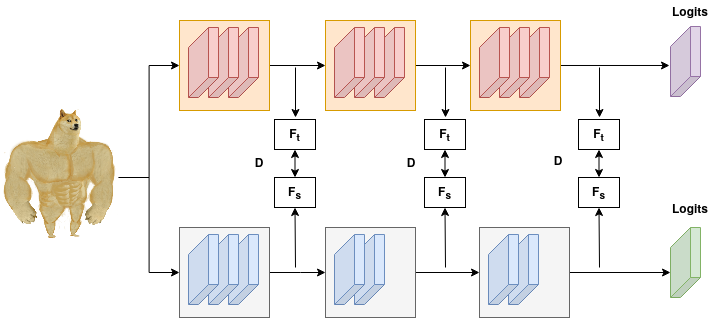
\includegraphics[width=0.8\linewidth]{assets/feature_based.png}
   \end{center}
      \caption{The typical architecture of feature-based knowledge distillation framework.}
   \label{fig:feature_base}
\end{figure*}